\section{Aturan Dasar Penulisan Kode PHP}
Seperti bahasa pemograman yang lain, PHP juga memiliki aturan penulisan seperti case sensitifity (perbedaan antara huruf besar dan kecil), cara mengakhiri sebuah baris perintah, dan pengaruh penggunakan spasi dalam membuat kode program PHP. Berikut adalah aturan dasar penulisan kode PHP:
\subsection{Case Sensitivity (perbedaan huruf besar dan kecil) dalam PHP}
PHP tidak membedakan huruf besar dan kecil (case insensitive) untuk penamaan fungsi (function), nama class, maupun keyword bawaan PHP seperti echo, while, dan class. Ketiga baris berikut akan dianggap sama dalam PHP:
\begin{lstlisting}
<?php
Echo “Hello World”;
ECHO “Hello World”;
EchO “Hello World”;
?>
\end{lstlisting}
Akan tetapi, PHP membedakan huruf besar dan huruf kecil (case sensitive) untuk penamaan variabel, sehingga akan dianggap sebagai variabel yang berbeda. Sering kali error terjadi dikarenakan salah menuliskan nama variabel, yang seharusnya menggunakan huruf kecil, ditulis dengan huruf besar.
\begin{lstlisting}
<?php
$luqman="Luqman";
echo $Luqman; // Notice: Undefined variable: Luqman
?>
\end{lstlisting}
Untuk mengatasi perbedaan ini, disarankan menggunakan huruf kecil untuk seluruh kode PHP, termasuk variabel, fungsi maupun class. Jika membutuhkan nama variabel yang terdiri dari 2 kata, karakter spasi bisa digantikan dengan underscore.
\subsection{Karakter Spasi dan Tab dalam PHP}
Dalam PHP, karakter seperti spasi dan tab diabaikan di dalam eksekusi program PHP. Anda boleh mencoba sebuah statement menjadi beberapa baris, atau menyatukan beberapa statement dalam sebuah baris yang lumayan panjang. Seperti contoh berikut:
\begin{lstlisting}
<?php
echo "Saya belajar"; echo "Saya mengerti"; $nama="Men";
?>
\end{lstlisting}
Baris statement itu sama dengan
 \begin{lstlisting}
<?php
     echo "Saya belajar";
     echo "Saya mengerti";
     $nama = "Men";
?>
\end{lstlisting}
Walaupun contoh yang pertama lebih menghemat baris, namun lebih disarankan untuk contoh kedua, karena kita mengusahakan agar setiap statement berada dalam satu baris saja, dan menambahkan beberapa spasi di awal untuk memudahkan membaca kode program.
\par
Keuntungan penghematan baris dan beberapa byte dari sebuah file PHP tidak akan sebanding dengan mencoba memahami kode program yang dibuat dalam beberapa hari kedepan. Menambahkan sebagian komentar pada bagian kode yang lebih rumit sebagai penjelasan juga sangat disarankan.
\section{Embedded Script dan Non Embedded}
\subsection{Embedded Script}
  \item Berikut merupakan contoh dokumen HTML yang akan dihasilkan dengan menggunakan program/script PHP dalam embedded script
    Ditampilkan dibawah ini  :
    \lstinputlisting[firstline=1, lastline=12]{src/embedded_script.php}
Script diatas menunjukkan contoh script PHP sederhana yang disebut dengan script embedded yang di sisipkan diantara tag-tag HTML. Script tersebut digunakan apabila isi dari suatu dokumen HTML diinginkan dari hasil eksekusi suatu script PHP. jika dilihat dari source-nya dengan menggunakan view source pada web browser maka tampilannya akan berupa seperti berikut
    \lstinputlisting[firstline=14, lastline=22]{src/embedded_script.php}
Source dokumen HTML yang tampil berupa dokumen HTML yang tidak lagi dari script PHP yang berisi script PHP karena semua menjadi tag HTML, karena pada saat dieksekusi maka bukan scriptnya yang dikirim tetapi eksekusi dari script tersebut yang dikirim 
\subsection{Non Embedded}
   \item Script PHP dibawah ini merupakan script murni dari pembuatan program dengan menggunakan PHP, tag dokumen HTML yang dihasilkan untuk membuat dokumen merupakan bagian dari script PHP. di tampilkan dibawah ini:
  \lstinputlisting[firstline=24, lastline=35]{src/embedded_script.php}
dan dibawah ini merupakan source dokumen HTML dari tampilan kode diatas  
  \lstinputlisting[firstline=38, lastline=40]{src/embedded_script.php}
Jika diperhatikan dokumen HTML tersebut tidak beraturan ditampilkan. Hal tersebut tidak menjadi masalah, yang penting adalah browser web dapat menampilkannya, karena dokumen tag HTML ini murni dihasilkan dari script PHP. 
\section{Variabel dan Tipe Data}
\subsection{Variabel}
Variabel adalah tempat penympanan data, variabel memiliki nama. dalam pemograman variabel merupakan tempat penyimpanan data didalam memori komputer. Didalam PHP nama variabel diawali dengan karakter dollar diikuti dengan huruf sebagai karakter pertama setelah dollar. kemudian kombinasi karakter dan angka. Tidak boleh ada spasi dan tanda baca dalam penamaannya. kecuali karakter (garis bawah, under score).berikut merupakan penulisan variabel yang benar:
\lstinputlisting[firstline=31, lastline=34]{src/tag_awal_akhir.php}
\subsection{Tipe Data}
Data yang diolah oleh suatu program memiliki berbagai jenis ada data yang menunjukkan jumlah dan menunjukkan nilai benar dan salah, atau tulisan. Jenis tipe data dalam PHP secara mendasar dibedakan menjadi 3 macam yang disebut sebagai tipe data primitif. Tipe data primitif yang diolah oleh PHP:
\begin{enumerate}
\item Numerik
\item String
\item Boolean
\end{enumerate}
Tipe data numerik dibedakan menjadi tipe data integer dan flooting point. Selain itu tipe data yang lain adalah tipe data compound, terdiri atas:
\begin{enumerate}
\item tipe data array
\item tipe data objek 
\end{enumerate}
\subsection{Tipe Data Integer}
 tipe data integer adalah tipe data yang terdiri dari angka bulat (tidak mengandung nilai pecahan atau nilai desimal). Nilai ini bisa berbentuk angka positif maupun negatif, contohnya 1, 2, 6, -44, 20000, atau 128730123. Tipe data integer dapat dituliskan dengan notasi sebagai berikut
\begin{enumerate}
\item Notasi Desimal adalah susunan bilangan yang mempunyai basis sepuluh. 
Koefisien bilangan desimal terdiri dari 0,1,2,3,4,5,6,7,8,9.
Notasi bilangan desimal dituliskan: (n)10
\item Notasi Oktal adalah susunan bilangan yang mempunyai basis delapan. 
Koefisien bilangan oktal terdiri dari 0,1,2,3,4,5,6,7.
Notasi bilangan oktal dituliskan : (n)8
\item Biner adalah susunan bilangan yang mempunyai basis dua. 
Basis dua di sini adalah nilai koefisien yaitu 0 dan 1.
Notasi bilangan biner dituliskan : (n)2
\item Notasi Heksadesimal adalah susunan bilangan yang mempunyai basis enam belas. 
Koefisien bilangan heksadesimal terdiri dari 0,1,2,3,4,5,6,7,8,9,A,B,C,D,F.

Catatan: A bernilai 10, B bernilai 11, ... , F bernilai 15.
Notasi bilangan hekasdesimal dituliskan : (n)16

\begin{figure}[!htbp]
 \centering
 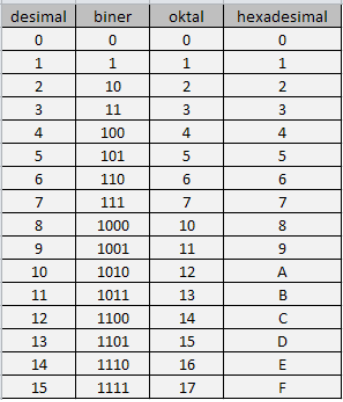
\includegraphics[width=.50\textwidth]{figures/sistem_bilangan.png}
 \caption{Sistem Bilangan}\label{fig:inputchapter}
\end{figure}

\end{enumerate}

\subsection{Tipe Data Floting Point}
Tipe data float (disebut juga tipe data floating point, atau real number) adalah tipe data angka yang memiliki bagian desimal di akhir angka, atau memiliki floating point (floating point adalah istilah dalam bahasa inggris untuk menyebut tanda “titik” yang menandakan bilangan desimal). Contoh angka float adalah seperti: 0,9 atau 3,14. Tipe data float cocok digunakan untuk variabel yang akan berisi angka pecahan, seperti nilai IPK, hasil pembagian, atau hasil komputasi numerik yang angkanya tidak bisa ditampung oleh data integer.
\subsection{Tipe Data String}
Tipe data String adalah tipe data untuk teks yang merupakan gabungan huruf, angka, whitespace (spasi), dan berbagai karakter. Fungsi ini digunakan untuk membuat identifier String/teks. Data string ditulis dengan mengapit data string tersebut dengan tanda petik tunggal atau tanda petik ganda. Tanda petik tunggal umumnya digunakan sebagai konstanta string.
\subsection{Tipe Data Boolean}
Tipe data boolean sebenarnya sangat sederhana. Tipe data ini hanya bisa diisi dengan salah satu dari 2 nilai: TRUE atau FALSE. Tipe data boolean banyak dipakai dalam percabangan kode program, atau untuk memutuskan apa yang harus dijalankan pada sebuah kondisi if else.
\subsection{Tipe Data Objek}
Tipe data dari objek merupakan tipe data baru, merupakan pengembangan PHP untuk mendukung program berorientasi objek. Tipe data objek adalah tipe data yang didalamnya mempunyai data dan method. data yang dipunyai oleh suatu objek populer dengan nama atribut dan method suatu objek umumnya berupa suatu fungsi. 

Data objek didefinisikan dengan membuat definisi kelas terlebih dahulu. Suatu variabel yang bertipe objek diinisialisasi (dideklarasi) dengan menggunakan perintah new kemudian nama objek (berupa nama kelas objek) berikut contohnya:
\lstinputlisting[firstline=1, lastline=17]{src/tipeDataObjek.php}


\section{Operator PHP}
Pada PHP, terdapat banyak operator  beberapa yang sering digunakan.
\subsection{Operator Perbandigan}
Seperti namanya, operator perbandingan digunakan untuk membandingkan beberapa buah nilai pada PHP dan hasilnya berupa booelan true yang berarti benar atau false yang berarti salah.
Contoh:
\begin{lstlisting}
<?php
if ($_POST['password'] == 'admin')
{
	echo 'Login sukses';
}
\end{lstlisting}

\subsection{ Operator PHP Increment dan Decrement}
Operator ini digunakan untuk menambahkan atau mengurangi nilai sebanyak 1 pada suatu variabel. 
\subsection{Perbedaan Pre Increment dan Post Increment}
Pada pre increment, nilai variabel akan ditambahkan 1 baru kemudian siap digunakan, sebaliknya, untuk  post increment, gunakan dulu nilai variabel kemudian baru ditambahkan dengan 1.
Contoh 1:
\begin{lstlisting}
<?php
$nomor = 1;
while($nomor <= 5) {
	echo $nomor++;
}
\end{lstlisting}
Contoh diatas akan menghasilkan angka 12345.

Contoh 2:
\begin{lstlisting}
<?php
$nomor = 1;
while($nomor <= 5) {
	echo ++$nomor;
}
\end{lstlisting}
Contoh diatas akan menghasilkan 23456.
Lihat, perbedaanya terdapat pada ++ sebelum dan sesudah $nomor. 

\subsection{Operator Assignment PHP}
Sesuai namanya Assignment operator ini digunakan untuk memberikan nilai pada suatu variabel. Operator dasarnya adalah tanda sama dengan ( = ). Dalam praktiknya, operator ini sering digunakan ketika menjumlahkan nilai pada suatu perulangan, seperti ketika menjumlahkan data hasil query database.
Contoh:
\begin{lstlisting}
<?php
$sql 	= 'SELECT * FROM sales';
$query 	= mysqli_query($sql);
$total	= 0;
while($row = mysqli_fetch_array($query))
{
	$total += $row['jml_bayar'];
}
\end{lstlisting}

\section{Struktur Kontrol}
PHP melakukan eksekusi dengan perintah mulai dari baris pertama kemudian ke baris berikutnya, sampai baris yang terakhir. Struktur kontrol digunakan dalam mengatur alur logika program agar sesuiai dengan kenyataan. Struktur kontrol akan melibatkan variabel, tipe data, dan operator. 
\subsection{If Statement}
If Statement  adalah pernyataan yang hanya akan dijalankan jika suatu kondisi bernilai benar, berfungsi untuk melakukan filter/penyaringan hasil berdasarkan kondisi tertentu. Contoh:
\begin{lstlisting}
If (kondisi) {
    Pernyataan 1;
    Pernyataan 2;
    .....
}else{
    Pernyataan a;
    Pernyataan b;
    .....
}
\end{lstlisting}
\subsection{Perulangan}
Perulangan digunakan untuk mengeksekusi suatu pernyataan secara berulang-ulang. Contoh:
\begin{lstlisting}
While (kondisi){
    Pernyataan yang diulang;
    Counter;
}
\end{lstlisting}
\subsection{Fungsi}
Fungsi adalah serangkaian kode yang terdapat kegunaan khusus dan tertentu, dengan adanya fungsi ini pemrograman dapat dipermudah karena tidak harus menulis berulang-ulang rangkian kode yang sama. Demikian juga dalam pengembangan, jika terjadi kesalahan atau perbaikan kode maka pemrogram hanya dapat melakukan perbaikan pada fungsi tertentu saja, tidak perlu melakukan perbaikan pada banyak kode. Contoh:
\begin{lstlisting}
$tanggal = date(“format”);
\end{lstlisting}
